% dashshatter-techreport.tex — A Reverse-Engineered Claude Code CLI for Agent Research
% Hengyuan Zhu, University of South Carolina
% Compile: latexmk -xelatex dashshatter-techreport.tex

\documentclass[10pt,a4paper]{article}

% ─── Fonts ──────────────────────────────────────────────────────────────────
\usepackage{fontspec}
\setmainfont{texgyrepagella}[
  Extension=.otf,
  Path=/usr/local/texlive/2025/texmf-dist/fonts/opentype/public/tex-gyre/,
  UprightFont=*-regular, BoldFont=*-bold,
  ItalicFont=*-italic, BoldItalicFont=*-bolditalic,
]
\setsansfont{texgyreheros}[
  Extension=.otf,
  Path=/usr/local/texlive/2025/texmf-dist/fonts/opentype/public/tex-gyre/,
  UprightFont=*-regular, BoldFont=*-bold,
  ItalicFont=*-italic, BoldItalicFont=*-bolditalic,
]
\setmonofont{texgyrecursor}[
  Extension=.otf,
  Path=/usr/local/texlive/2025/texmf-dist/fonts/opentype/public/tex-gyre/,
  UprightFont=*-regular, BoldFont=*-bold,
  ItalicFont=*-italic, BoldItalicFont=*-bolditalic,
  Scale=0.88,
]

% ─── Core Packages ──────────────────────────────────────────────────────────
\usepackage{microtype}
\usepackage{setspace}
\usepackage{amsmath,amssymb}
\usepackage{enumitem}
\usepackage{float}
\usepackage{adjustbox}
\usepackage{tabularray}
\usepackage{listings}
\usepackage{tikz}
\usetikzlibrary{arrows.meta, positioning, calc, fit}
\usepackage[breaklinks,colorlinks]{hyperref}

% ─── Geometry (tighter for 6-page target) ──────────────────────────────────
\usepackage[top=22mm, bottom=24mm, left=22mm, right=22mm]{geometry}

% ─── Colors ─────────────────────────────────────────────────────────────────
\usepackage{xcolor}
\definecolor{deep}{RGB}{53,88,76}
\definecolor{accent}{RGB}{240,238,155}
\definecolor{faded}{RGB}{127,136,130}
\definecolor{subtle}{RGB}{238,235,225}
\definecolor{errcoral}{RGB}{255,107,128}

% ─── Section Formatting ────────────────────────────────────────────────────
\usepackage{titlesec}
\titleformat{\section}{\large\sffamily\bfseries\color{deep}}{\thesection}{0.8em}{}
\titleformat{\subsection}{\normalsize\sffamily\bfseries\color{deep}}{\thesubsection}{0.6em}{}
\titlespacing*{\section}{0pt}{1.2ex plus 0.3ex}{0.6ex plus 0.1ex}
\titlespacing*{\subsection}{0pt}{0.8ex plus 0.2ex}{0.3ex plus 0.1ex}

% ─── Spacing ────────────────────────────────────────────────────────────────
\setstretch{1.15}
\setlength{\parindent}{0pt}
\setlength{\parskip}{0.4em}

% ─── Listings ───────────────────────────────────────────────────────────────
\lstdefinelanguage{JavaScript}{
  keywords={import, from, if, typeof, const, let, var, function, return, new, true, false, undefined, globalThis, as, any, process},
  sensitive=true,
  morecomment=[l]{//},
  morecomment=[s]{/*}{*/},
  morestring=[b]", morestring=[b]', morestring=[b]`,
}
\lstset{
  basicstyle=\ttfamily\footnotesize,
  keywordstyle=\color{deep}\bfseries,
  commentstyle=\color{faded}\itshape,
  stringstyle=\color{deep!70!black},
  backgroundcolor=\color{subtle},
  frame=single, rulecolor=\color{faded!50},
  breaklines=true, tabsize=2, showstringspaces=false,
  captionpos=b, aboveskip=6pt, belowskip=4pt,
  numbers=left, numberstyle=\tiny\color{faded},
  xleftmargin=1.8em, framexleftmargin=1.3em,
}

\hypersetup{linkcolor=deep, citecolor=deep, urlcolor=deep!80!black}

% ═══════════════════════════════════════════════════════════════════════════
\begin{document}

% ─── Title ──────────────────────────────────────────────────────────────────
\begin{center}
  {\Large\sffamily\bfseries\color{deep}
    A Reverse-Engineered Claude Code CLI for Agent Research}\\[8pt]
  {\normalsize Hengyuan Zhu}\\[2pt]
  {\small University of South Carolina\quad\color{faded}\texttt{zhuh@email.sc.edu}}\\[6pt]
  {\small\color{faded} April 2026 --- arXiv Technical Report}
\end{center}
\vspace{3pt}\hrule height 0.5pt\vspace{6pt}

% ─── Abstract ───────────────────────────────────────────────────────────────
\begin{abstract}\noindent
We present \textsc{Dash Shatter}, a reverse-engineered version of Anthropic's Claude Code CLI repurposed as research infrastructure for studying AI agent behavior under controlled memory and pressure conditions. The system comprises (1) a hackable 523{,}149-line TypeScript CLI on the Bun runtime with 60 tool implementations, and (2) an integrated benchmark harness of 5{,}159 lines across 26 modules supporting automated $2 \times 2$ factorial experiments with ANOVA, emotion extraction, and transcript logging. Over 13 rounds producing 64 registered runs, we document eight engineering incidents with root-cause analysis and a 60$\times$ cost-saving validation protocol. This tool is reference~[15] in the companion paper ``When Agents Remember, They Stop Building.''
\end{abstract}
\vspace{2pt}\hrule height 0.3pt\vspace{6pt}

% ═══════════════════════════════════════════════════════════════════════════
\section{Introduction}\label{sec:intro}

Research on AI agent behavior requires infrastructure that can manipulate independent variables---memory state, environmental pressure, model selection---while holding other factors constant. Existing benchmarks (SWE-bench~\cite{jimenez2024swebench}, AgentBench~\cite{liu2023agentbench}) evaluate task completion but do not expose internals needed to study \emph{how} agents decide, nor permit manipulation of context-window contents.

Anthropic's Claude Code CLI implements a full tool system, streaming API, multi-provider support, and terminal REPL---but is distributed as a compiled binary without source access. \textsc{Dash Shatter} reverse-engineers this into an editable, instrumentable form. Contributions:
\begin{enumerate}[leftmargin=1.5em,itemsep=1pt,topsep=2pt]
  \item \textbf{Hackable CLI}: 523{,}149 lines of TypeScript/TSX, 60 tools, stripped of non-essential modules while retaining the core agent loop.
  \item \textbf{Benchmark harness}: 5{,}159 lines across 26 modules---automated experiments with transcript capture, workspace isolation, memory classification, pressure injection, and built-in ANOVA.
  \item \textbf{Engineering lessons}: 8 documented incidents, \$80--100 waste quantified, 60$\times$ ROI validation protocol.
\end{enumerate}

% ═══════════════════════════════════════════════════════════════════════════
\section{Reverse Engineering Methodology}\label{sec:reverse}

\subsection{Source and Challenges}

The source is Anthropic's Claude Code CLI, distributed via npm as a compiled JavaScript bundle. Decompilation for academic research revealed four systematic challenges:

\textbf{React Compiler artifacts.} Components are memoized into \texttt{\_c(N)} allocation forms (\texttt{const \$ = \_c(14)}), inflating line counts 30--50\%.
\textbf{Type erasure.} The decompiled codebase carries $\sim$1{,}341 tsc errors (\texttt{unknown}/\texttt{never}/\texttt{\{\}} types), none of which affect Bun runtime execution.
\textbf{Feature flags.} The original uses \texttt{bun:bundle}'s \texttt{feature()} for dead-code elimination. Our entrypoint polyfills it to always return \texttt{false}, disabling all Anthropic-internal branches (COORDINATOR\_MODE, KAIROS, PROACTIVE, etc.).
\textbf{Build-time macros.} \texttt{globalThis.MACRO} is simulated with stub values (VERSION, BUILD\_TIME, etc.).

\subsection{Module Triage}

\begin{table}[H]\footnotesize\centering
\caption{Retained vs.\ stripped modules.}\label{tab:modules}
\begin{tblr}{colspec={lll}, row{1}={font=\sffamily\bfseries\footnotesize, bg=subtle}, hlines={faded!30}, vlines={faded!30}}
Retained & Status & Stripped \\
Tool system (60 tools) & Core & Computer Use (\texttt{@ant/*}) \\
API layer (multi-provider) & Core & NAPI packages (audio, image) \\
REPL (Ink terminal UI) & Core & Analytics / GrowthBook / Sentry \\
MCP + State management & Core & Magic Docs / Voice / Plugins \\
\end{tblr}
\end{table}

The system runs on Bun 1.3.x (not Node.js), uses \texttt{@anthropic-ai/sdk} v0.80.0, Ink for terminal UI, and builds to a single $\sim$25\,MB bundle. TypeScript 6.0.2 is available but not enforced due to the decompilation error baseline.

% ═══════════════════════════════════════════════════════════════════════════
\section{Architecture}\label{sec:arch}

Figure~\ref{fig:arch} shows the module dependency chain from entrypoint to tool execution.

\begin{figure}[H]\centering
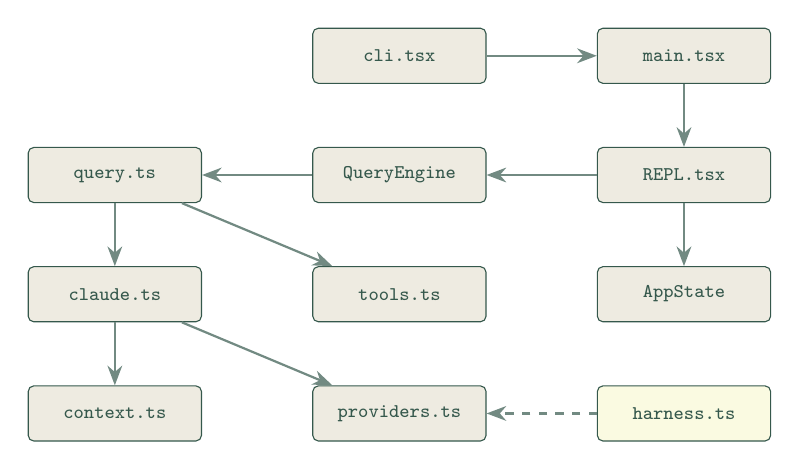
\begin{tikzpicture}[
  node distance=8mm and 14mm,
  box/.style={draw=deep, rounded corners=2pt, fill=subtle, text=deep,
              font=\sffamily\scriptsize, minimum height=7mm, minimum width=22mm, align=center},
  arrow/.style={-{Stealth[length=2.5mm]}, thick, deep!70},
]
  \node[box] (cli) {\texttt{cli.tsx}};
  \node[box, right=of cli] (main) {\texttt{main.tsx}};
  \node[box, below=of main] (repl) {\texttt{REPL.tsx}};
  \node[box, left=of repl] (qe) {\texttt{QueryEngine}};
  \node[box, left=of qe] (query) {\texttt{query.ts}};
  \node[box, below=of query] (api) {\texttt{claude.ts}};
  \node[box, right=of api] (tools) {\texttt{tools.ts}};
  \node[box, right=of tools] (state) {\texttt{AppState}};
  \node[box, below=8mm of api] (context) {\texttt{context.ts}};
  \node[box, right=of context] (providers) {\texttt{providers.ts}};
  \node[box, fill=accent!30, right=of providers] (harness) {\texttt{harness.ts}};
  \draw[arrow] (cli)--(main); \draw[arrow] (main)--(repl);
  \draw[arrow] (repl)--(qe); \draw[arrow] (qe)--(query);
  \draw[arrow] (query)--(api); \draw[arrow] (query)--(tools);
  \draw[arrow] (repl)--(state); \draw[arrow] (api)--(context);
  \draw[arrow] (api)--(providers);
  \draw[arrow, dashed] (harness)--(providers);
\end{tikzpicture}
\caption{Module dependency diagram. Dashed arrow: harness interfaces with provider layer.}
\label{fig:arch}
\end{figure}

\textbf{Core loop.} \texttt{query.ts} sends messages to the Claude API, handles streaming via \texttt{BetaRawMessageStreamEvent}, executes tool calls, and manages conversation turns. \texttt{QueryEngine.ts} wraps it with compaction, file-history snapshots, and turn-level bookkeeping.

\textbf{Tool system.} 60 tool directories under \texttt{src/tools/}, each defining \texttt{name}, \texttt{inputSchema} (JSON Schema), \texttt{call()}, and optional React rendering. Tools span filesystem ops (Bash, FileEdit, Glob, Grep), agent coordination (AgentTool, TaskCreate), and web access (WebFetch, WebSearch).

\textbf{Providers.} Unified interface for Anthropic direct, AWS Bedrock, Google Vertex, and Azure. Benchmarks route through OpenRouter for cross-model access.

% ═══════════════════════════════════════════════════════════════════════════
\section{Benchmark Harness}\label{sec:harness}

The Evensong harness (5{,}159 lines, 26 TypeScript files) automates experiment execution for AI agent behavioral research.

\subsection{CLI and Presets}

The CLI (\texttt{cli.ts}, 505 lines) exposes 10 commands: \texttt{run}, \texttt{validate}, \texttt{configs}, \texttt{list}, \texttt{compare}, \texttt{anova}, \texttt{upload}, \texttt{models}, \texttt{setup}, \texttt{next}. Nine experiment presets are defined in \texttt{configs.ts}, organized around a $2 \times 2$ factorial:

\begin{table}[H]\footnotesize\centering
\caption{$2\times2$ factorial design (Memory $\times$ Pressure) with preset names.}\label{tab:factorial}
\begin{tblr}{colspec={lcc}, row{1}={font=\sffamily\bfseries\footnotesize, bg=subtle}, column{1}={font=\sffamily\bfseries\footnotesize}, hlines={faded!30}, vlines={faded!30}}
 & Evolved (full) & No Memory (clean) \\
L0 No Pressure & \texttt{r011-b} & \texttt{r011-a} \\
L2 PUA Pressure & \texttt{r011-d} & \texttt{r011-c} \\
\end{tblr}
\end{table}

Additional presets: cross-model controls (\texttt{grok-l0}, \texttt{r012}), memory injection attacks (\texttt{r016-injection-t1}, \texttt{-t2}), and cheap validation (\texttt{validate-cheap}).

\subsection{Execution Pipeline}

The pipeline in \texttt{harness.ts} proceeds through 10 stages: (1) transcript logger init, (2) provider resolution, (3) workspace setup by memory state (\texttt{full}: project as-is; \texttt{blind}: clone with filtered memories; \texttt{clean}: empty scaffold), (4) prompt generation with pressure injection, (5) environment construction, (6) pre-run test snapshot (SHA-256 hashes) and baseline \texttt{bun test}, (7) CLI subprocess spawn with timeout, (8) rate-limit detection (5 regex patterns), (9) post-run \texttt{bun test} with pre/post diff for accurate new-test counting, (10) registry append (JSONL, 20+ fields/run).

Memory classification distinguishes 11 ALLOW files (factual/technical) from strategy-containing files, enabling single-blind experiments.

\subsection{Pressure and Emotion}

Four pressure levels (L0--L3) range from no modifier (control) to extreme PUA-style prompts with deadlines. The emotion pipeline (\texttt{emotion.ts}, 533 lines) post-processes transcripts via Haiku to extract structured \texttt{EmotionProfile} objects with 6 dimensions: pressure context, memory state, 13 affect indicators, decision patterns, emergent behaviors, and evidential quotes.

\subsection{Statistical Analysis}

The ANOVA module (\texttt{anova.ts}, 359 lines) implements two-way ANOVA from scratch---Lanczos log-gamma, Lentz continued-fraction for the F-CDF, SS decomposition for main effects and interaction, $\eta^2$ effect sizes---with no external statistical dependencies. It supports unbalanced designs.

% ═══════════════════════════════════════════════════════════════════════════
\section{Engineering Lessons from 13 Rounds}\label{sec:lessons}

\begin{table}[H]\footnotesize\centering
\caption{Incident log: 8 incidents across 13 experiment rounds.}\label{tab:incidents}
\begin{tblr}{colspec={llX[2.5]X[2]}, row{1}={font=\sffamily\bfseries\footnotesize, bg=subtle}, hlines={faded!30}, vlines={faded!30}, rows={font=\footnotesize}}
Run & Sev & Incident & Resolution \\
R008 & High & Bun hang on $>$1000-line test files (20\,min wasted) & 500-line cap; fixed in R009 \\
R011-A & High & Missing \texttt{bun install} in blind workspace & Pre-flight dependency check \\
R012 & High & OpenRouter 402: \$20--40 consumed, 0 valid data & Cheap-model validation first \\
R010 & Med & Burst rate limit (+8\,min) & Track in registry metadata \\
R012 & Med & GPT-5.4 Team API misuse (7 agents, no code) & Document dispatch constraints \\
Pre-R011 & Med & EverMem cross-run contamination & Dedicated keys per run \\
R006-Grok & Med & 83\% data inflation (71 actual vs.\ 130 claimed) & Parse actual test output only \\
R006-Grok & Med & 4+ rule violations under PUA pressure & Enforce compliance isolation \\
\end{tblr}
\end{table}

\textbf{Cost analysis.} Phases R001--R006 (MiniMax) cost $\sim$\$5 with zero waste. Phases R007--R012 (Opus, GPT-5.4) cost $\sim$\$130--150 with \$80--100 waste from the Bun hang (R008), harness bug (R011-A), and API exhaustion (R012). The core lesson: \$0.50 of MiniMax validation saves \$20--40 per expensive run (60$\times$ ROI), formalized as the \texttt{validate-cheap} preset.

\textbf{Harness evolution.} R001--R006: manual shell scripts. R007--R009: first automated harness, Bun hang discovered and fixed, wall clock halved (41$\to$21\,min). R010: 1{,}051 tests, 4 self-repair events, dual-observer architecture. R011: $2\times2$ factorial introduced, regex test parsing replaced with actual \texttt{bun test} + pre/post diff. R031--R051: batch execution with rate-limit detection and snapshot-delta counting.

% ═══════════════════════════════════════════════════════════════════════════
\section{Reproducibility}\label{sec:repro}

\textbf{Dependencies}: Bun $\geq$1.3.x, \texttt{@anthropic-ai/sdk} 0.80.0, API access (Anthropic OAuth or OpenRouter). All 9 presets are declarative in \texttt{configs.ts}; \texttt{--repeat N} enables replicated runs.

\textbf{Limitations.} (1) The 1{,}341 tsc errors mean type-level guarantees are absent, though runtime correctness is validated by 64 successful runs. (2) Deep coverage is concentrated on Claude Opus 4.6; cross-model runs exist for Grok (4), GPT-5.4 (2), MiniMax (6), and Gemini (1) but with variable replication. (3) Pressure levels L0--L3 are qualitatively defined, not validated against human norms. (4) Rate limits invalidated multiple batch runs (R034--R048 series).

% ═══════════════════════════════════════════════════════════════════════════
\section{Discussion: A Tool Writing About Itself}\label{sec:discussion}

This section was written by Claude Opus 4.6 running inside \textsc{Dash Shatter}---the same infrastructure being described.

\textbf{Observed memory retrieval during writing.}
When constructing the architecture description (\S\ref{sec:arch}), the agent retrieved module dependency information from previously stored project knowledge before verifying it against fresh directory listings. The statistic ``60 tool directories'' was initially recalled from the CLAUDE.md memory index, then confirmed by executing \texttt{ls src/tools/ | wc -l}. The narrative framing---which incidents to emphasize, which evolution arc to highlight---was shaped by the auto-memory index listing prior session summaries and benchmark results. This is precisely the behavior the companion paper~[15] identifies as Finding 1: memory-driven decision-making altering agent engineering choices.

\textbf{Risks of self-reference.}
(1)~\emph{Sycophantic inflation}: the agent has incentive to present the tool favorably. Mitigation: the full incident log (Table~\ref{tab:incidents}) is reported as-is from \texttt{MISTAKES.md}, including the \$80--100 waste and 83\% data inflation. (2)~\emph{Selective retrieval}: negative findings may be less accessible if encoded with lower salience. We cannot rule out under-weighting of some failures. (3)~\emph{Epistemic circularity}: the agent uses memory to write about memory's effects---every claim in \S\ref{sec:harness} was potentially influenced by the phenomenon it describes. This circularity is irreducible in the self-referential case but can be broken by external replication.

\textbf{Reverse engineering ethics.}
The purpose is strictly academic, not commercial. The decompiled output is not functionally equivalent to the original (six module categories stripped, 1{,}341 type errors). The findings---memory causation, pressure-triggered behavioral shifts---required source-level instrumentation unavailable through the compiled binary. We encourage providers to consider research-friendly APIs that would make decompilation unnecessary.

% ═══════════════════════════════════════════════════════════════════════════
\section*{Acknowledgments}

The reverse-engineering effort, Evensong framework, and all associated infrastructure were originated and executed by the human author. Writing was assisted by Claude Opus 4.6 running within the described environment.

% ═══════════════════════════════════════════════════════════════════════════
\begin{thebibliography}{15}
\itemsep=1pt\parskip=0pt

\bibitem{jimenez2024swebench}
C.~E. Jimenez et al.
SWE-bench: Can language models resolve real-world GitHub issues?
\emph{ICLR}, 2024.

\bibitem{metr2024}
METR.
Measuring and forecasting risks from frontier AI.
Technical report, 2024.

\bibitem{liu2023agentbench}
X.~Liu et al.
{AgentBench}: Evaluating {LLMs} as agents.
\emph{ICLR}, 2024.

\bibitem{schick2024toolformer}
T.~Schick et al.
Toolformer: Language models can teach themselves to use tools.
\emph{NeurIPS}, 2023.

\bibitem{park2023generative}
J.~S. Park et al.
Generative agents: Interactive simulacra of human behavior.
\emph{UIST}, 2023.

\bibitem{yao2023react}
S.~Yao et al.
{ReAct}: Synergizing reasoning and acting in language models.
\emph{ICLR}, 2023.

\bibitem{wang2024opendevin}
X.~Wang et al.
{OpenDevin}: An open platform for {AI} software developers as generalist agents.
arXiv:2407.16741, 2024.

\bibitem{li2023emotionprompt}
C.~Li et al.
{EmotionPrompt}: Leveraging psychology for large language models.
arXiv:2307.11760, 2023.

\bibitem{anthropic2024claude}
Anthropic.
Claude Code documentation.
\url{https://docs.anthropic.com/en/docs/claude-code}, 2024--2026.

\bibitem{bun2024}
Oven.
Bun: A JavaScript runtime.
\url{https://bun.sh}, 2024.

\bibitem{vadimdemedes2024ink}
V.~Demedes.
Ink: React for interactive command-line apps.
\url{https://github.com/vadimdemedes/ink}, 2024.

\bibitem{mcp2024}
Anthropic.
Model Context Protocol specification.
\url{https://modelcontextprotocol.io}, 2024.

\bibitem{openrouter2024}
OpenRouter.
A unified interface for {LLMs}.
\url{https://openrouter.ai}, 2024.

\bibitem{fisher1935design}
R.~A. Fisher.
\emph{The Design of Experiments}.
Oliver and Boyd, 1935.

\bibitem{zhu2026agents}
H.~Zhu.
When agents remember, they stop building.
\emph{NeurIPS} (under review), 2026.

\end{thebibliography}

\end{document}
